\documentclass[../opis-rozwiazania.tex]{subfiles}

\begin{document}

\label{diagrams:activity_diagrams}

\subsection{Uzyskanie sesji}

Proces opisuje prośbę klienta o~ustanowienie dla niego sesji. Sesja może już istnieć lub zostać dopiero utworzona.

\begin{figure}[H]
  \centering
  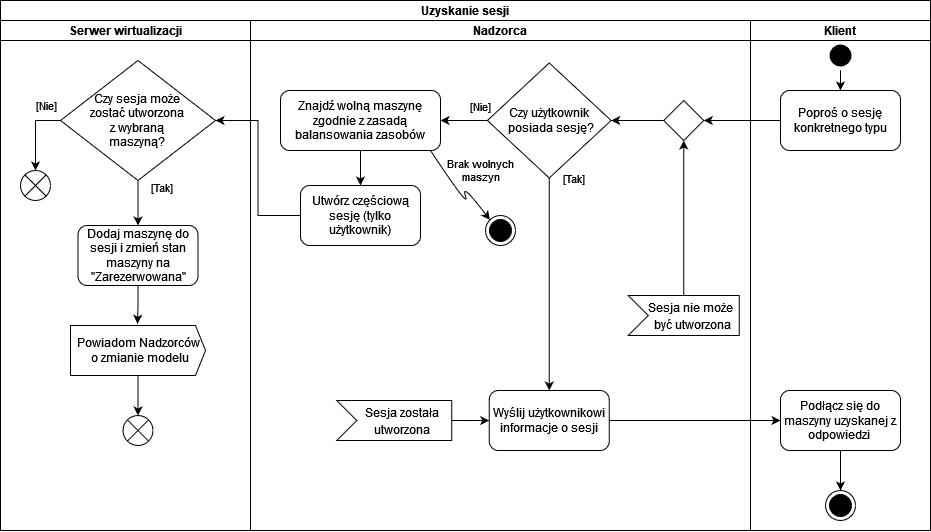
\includegraphics[width=\textwidth]{../diagrams/activity_diagrams/uzyskanie_sesji_v2.png}
  \caption{Proces uzyskania sesji}
  \label{start_session}
\end{figure}

Jeżeli sesja już istnieje, to zostaje zwrócona użytkownikowi.
W~przeciwnym razie nadzorca, na podstawie modelu systemu, wybiera pewną wolną maszynę i~wysyła do serwera wirtualizacji, na którym działa wybrana maszyna, prośbę o~utworzenie sesji.
Możliwość działania wielu nadzorców wymaga, aby proces ten był powtarzalny.
Czyli dla konkretnego stanu modelu musi zawsze zostać wybrana ta sama maszyna.
W~przypadku braku wolnej maszyny użytkownikowi zgłoszony jest błąd.
Z~założenia taka sytuacja może zajść jedynie, gdy wszystkie maszyny zostały zajęte i~brakuje zasobów na utworzenie nowych. Wynika to z~tego, że system powinien w~miarę możliwości trzymać pewien zapas wolnych maszyn.
Może się zdarzyć, że model jest nieaktualny i~nie można utworzyć sesji z~wcześniej wybraną maszyną.
Taka prośba zostaje odrzucona przez serwer wirtualizacji, ale odświeżenie modelu spowoduje powtórzenie procesu, tym razem wybierając inną maszynę.

Uzyskanie sesji przez użytkownika zrealizowane jest asynchronicznie.
Użytkownik oddzielnym zapytaniem prosi o~uzyskanie sesji, po czym używając otrzymanego identyfikatora sesji prosi o~jej dane.
Obiekt jest w~pełni utworzony, gdy odpowiedź nadzorcy zawiera sesję w~stanie gotowym oraz adres przypisanej maszyny.

\subsection{Kończenie sesji}

Proces ma za zadanie zakończyć sesję oraz wyłączyć skojarzoną z~nią wirtualną maszynę w~celu zwolnienia zasobów.

\begin{figure}[H]
  \centering
  \includegraphics[width=0.8\textwidth]{../diagrams/activity_diagrams/kończenie_sesji.png}
  \caption{Proces zakończenia sesji}
  \label{finish_session}
\end{figure}

Proces rozpoczyna się w~momencie, gdy użytkownik odłączy się od systemu lub utraci połączenie. Po upłynięciu ustalonego czasu, jeżeli użytkownik nie podłączył się ponownie, maszyna zostaje wyłączona.
Serwer wirtualizacji informuje nadzorcę o~utracie połączenia lub odłączeniu się użytkownika poprzez zmianę modelu.
Decyzję o~wyłączeniu maszyny podejmuje nadzorca.
Powoduje to, że zmiana konfiguracji aplikacji nadzorczych będzie oznaczać spójną reakcje całego systemu.

\subsection{Rozpoczęcie pracy serwera wirtualizacji}

Proces opisuje przyjęcie nowego serwera wirtualizacji do systemu.

\begin{figure}[H]
  \centering
  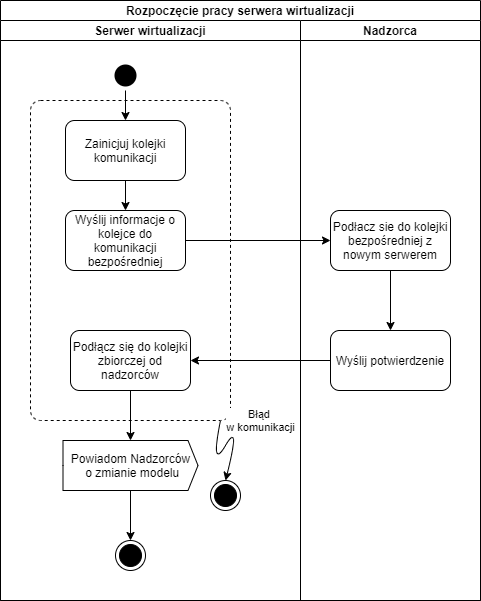
\includegraphics[width=0.8\textwidth]{../diagrams/activity_diagrams/serwer_start.png}
  \caption{Proces rozpoczęcia pracy serwera wirtualizacji}
  \label{start_virtsrv}
\end{figure}

Serwer wirtualizacji bez działającego nadzorcy nie jest w~stanie obsługiwać użytkowników.
Oznacza to, że jeśli przy starcie nie wykryje brokera wiadomości
lub nadzorcy po drugiej stronie kolejek \parencite{rabbit-ack} to się wyłączy.
Jeżeli jednak komunikacja z~nadzorcą jest możliwa, to serwer podłączy się do wspólnych kolejek (rozdział \ref{modules:broker}, kolejka \ref{modules:broker:queue-virtsrv})
oraz prześle informację o~kolejce bezpośredniej (rozdział \ref{modules:broker}, kolejka \ref{modules:broker:queue-exclusive}).
Gdy komunikacja będzie ustanowiona bezwarunkowo wyśle stan swojego modelu do nadzorców.

\end{document}